\documentclass[12pt]{article}
\usepackage{amsmath}
\usepackage{graphicx,psfrag,epsf}
\usepackage{enumerate}
\usepackage{algorithm}
\usepackage{algorithmicx}
\usepackage{algpseudocode}
\usepackage{xcolor}
\usepackage{natbib}
\usepackage{url} % not crucial - just used below for the URL 
\usepackage{nameref}
\usepackage{listings}

%\pdfminorversion=4
% NOTE: To produce blinded version, replace "0" with "1" below.
\newcommand{\blind}{0}
\newcommand{\factorMerger}{\textbf{factorMerger }}
\newcommand{\todo}{\textcolor{red}}
\newcommand{\M}{\mathcal{M}}
\newcommand{\code}{\texttt}

% DON'T change margins - should be 1 inch all around.
\addtolength{\oddsidemargin}{-.5in}%
\addtolength{\evensidemargin}{-.5in}%
\addtolength{\textwidth}{1in}%
\addtolength{\textheight}{1.3in}%
\addtolength{\topmargin}{-.8in}%


\begin{document}

%\bibliographystyle{natbib}

\def\spacingset#1{\renewcommand{\baselinestretch}%
{#1}\small\normalsize} \spacingset{1}


%%%%%%%%%%%%%%%%%%%%%%%%%%%%%%%%%%%%%%%%%%%%%%%%%%%%%%%%%%%%%%%%%%%%%%%%%%%%%%

\if0\blind
{
  \title{\bf Merging paths plots: A likelihood based visualisation of k-sample adaptive fusing}
  \author{Agnieszka Sitko\thanks{
    \todo{The authors gratefully acknowledge}}\hspace{.2cm}\\
    Faculty of Mathematics,  
    Informatics and Mechanics \\
    University of Warsaw\\
    and \\
    Przemys\l{}aw Biecek \\
    Faculty of Mathematics and Information Science,\\
	Warsaw University of Technology\\
    Faculty of Mathematics,  
    Informatics and Mechanics \\
    University of Warsaw}
  \maketitle
} \fi

\bigskip
\begin{abstract}

In this article we introduce \textbf{factorMerger} - a methodology and a software package for exploration and visualisation of k-group comparisons. Comparison of k-groups is one of the most important issues in exploratory analyses and is has zillions of applications. The classical solution is to test the global hypothesis, that all groups are equal. If the global null hypothesis is rejected a more detailed analysis of differences among pairs of groups is needed. The traditional approach is to perform \emph{post hoc tests} in order to verify which groups differ significantly. But this approach fails with large number of groups. This is why \textbf{factorMerger} is needed to concisely summarize group differences. 

\todo{The text of your abstract.  200 or fewer words.}
\end{abstract}

\noindent%
{\it Keywords:}  \textit{One-way analysis of variance}, post-hoc testing, hierarchical clustering, likelihood ratio test 
\vfill

\newpage
\spacingset{1.45} % DON'T change the spacing!
\section{Introduction and Motivation}
\label{sec:intro}
One of the most important issues in exploratory analyses is the comparison of k-groups. There are zillions of applications, like comparisons of different medical treatments, comparisons of different countries, or comparisons of segments of clients. The classical solution is to test the global hypothesis, that all groups are equal. 
If the global null hypothesis is rejected a more detailed analysis of differences among pairs of groups is needed. The traditional approach is to perform \emph{post hoc tests} in order to verify which groups differ significantly. 

As we show later, this approach fails if the number of groups is large as the number of pairs quickly grow beyond easy interpretation.  This is why in this article we introduce \textbf{factorMerger} - a methodology and a software package for exploration and visualisation of k-group comparisons. 

The larger is the number of groups, the more pronounced is the problem with classical post-hoc testing. 
For example, in the PISA study \citep{pisa2012} we have data about academic performance of 15-years old kids from 65 countries. One can use tests like ANOVA or other k-sample tests to verify whatever there are any differences between countries but then the question arises how counties are different. The total number of pairwise comparison is $\frac{65(65-1)}{2}=2080$ and obviously it is not easy to present such a number of results in an easy to understand way. Figure \ref{fig:postHocPISA} shows how hard is to read anything when the number of groups is large.

And the problem with post-hoc testing is also related to the inconsistency of results. For a fixed significance level, it is possible that the mean in group A does not differ significantly from the one in group B, similarly with groups B and C. At the same time the difference between group A and C is detected. Then data partition is unequivocal and, as a consequence, impossible to put through. 

To deal with this problem, we introduce the \emph{Merging Paths Plots} along with a tool - \textbf{factorMerger} - an R package \citep{Rcran}. The aim of this plot is to enrich results from \emph{k-sample} tests together with providing the variety of plots designed for deeper understanding analyzed models. 
An example of MPP plot is presented in Figure \ref{fig:FMtukeydone2}.

\begin{figure}[h!tbp]
\centering
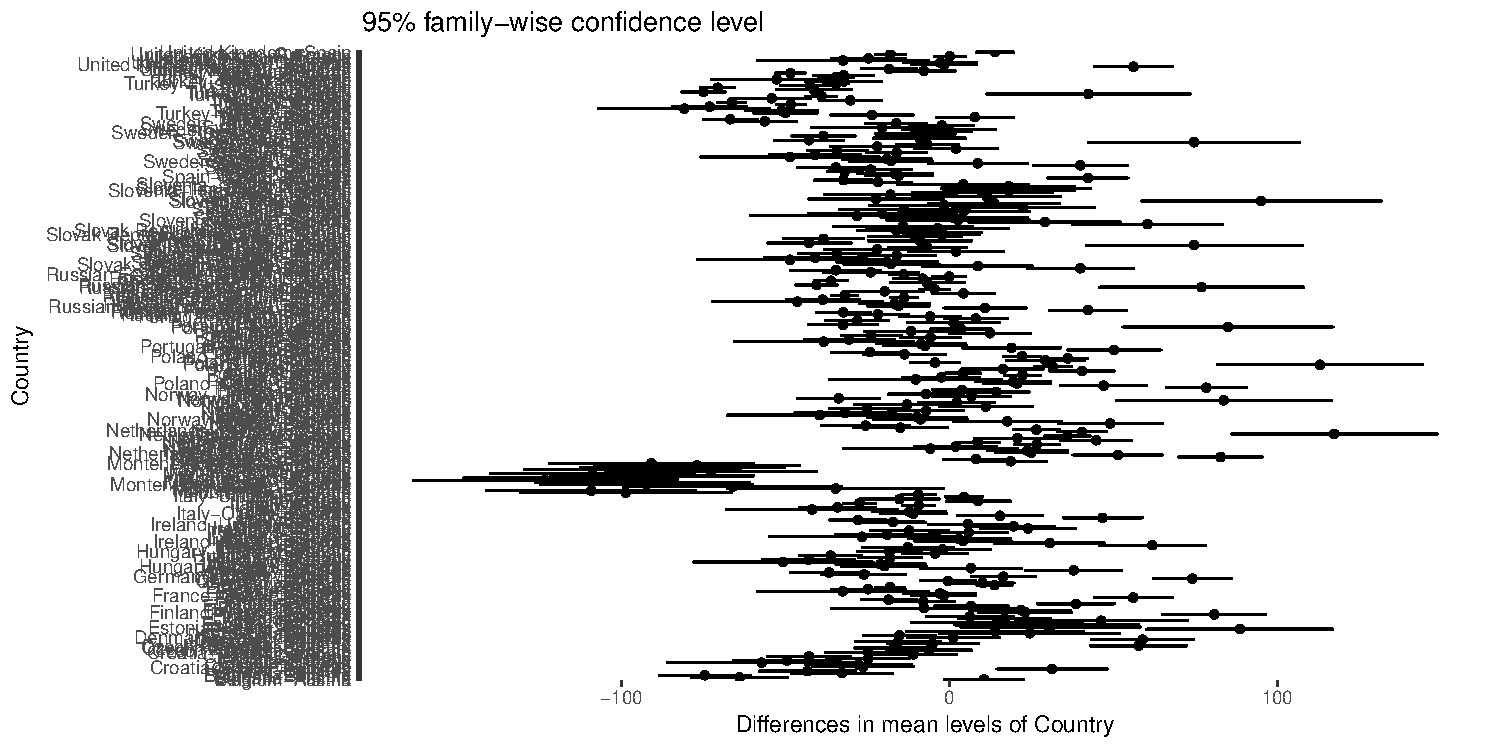
\includegraphics[scale=0.6]{PISA_post_hoc}
\caption{\label{fig:postHocPISA}\todo{ASI: przygotuj wykres dla wszystkich par krajow przedstawionych na rysunku 2.} Classical approach to graphical presentation of post-hoc testing of 11 groups. Here the data from PISA 2012 study is presented. For 11 counties there are 55 pairs. For each pair of countries the plot presents average difference and a confidence interval.}
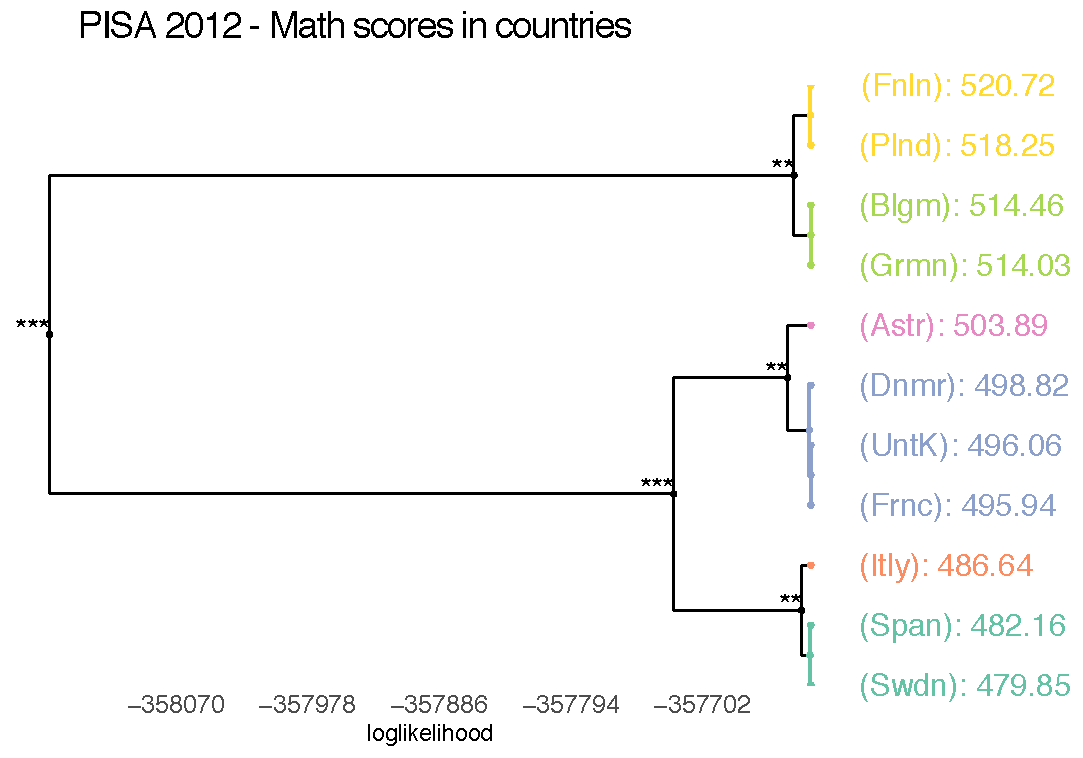
\includegraphics[scale=0.6]{FM_tukey_done2}
\caption{\label{fig:FMtukeydone2}Structure of similarity in academic performance among 11 countries may be alternatively presented with Merging Paths Plots. Such plot is much easier to read and interpret than the Figure \ref{fig:postHocPISA}.}
\end{figure}

\clearpage

The aim of \factorMerger package is to provide an informative and easy to understand visualizations of post-hoc comparisons. 
It works for wide spectrum of probability distribution families of dependent variable, like Gaussian or binomial distribution, works also for censored variables. 
The \emph{Merging Paths Plots} shows consistent and non-overlapping adaptive fusing of groups based on the likelihood ratio test (LRT) statistics. 
In addition, the Generalized Information Criterion (GIC) is presented for fused models. This criterion may be used to choose the optimal fusion of groups. 

\section{Background and Related Work}

One may find implementations of the traditional \emph{post hoc tests} in many \emph{R} packages (\cite{Rcran}). For example, package \textbf{agricolae} \citep{Agric} offers a wide range of them. It gives one of the most popular \emph{post hoc test}, Tukey HSD test (function \code{HSD.test}), its less conservative version --- Student-Newman-Keuls test (function \code{SNK.test}) or Scheffe test (function \code{scheffe.test}) which is robust to group imbalance. These parametric tests are based on Student's t-distribution, thus, are reduced to Gaussian models only. In contrasts, \textbf{multcomp} package \citep{Multcomp} can be used with generalized linear models (function \code{glht}) as it uses general linear hypothesis. Similarly to the \textbf{multcomp}, some implementations that accept \code{glm} objects are also given in \textbf{car} (\code{linearHypothesis}, \citealp{car}) and \textbf{lsmeans} \citep{lsmeans}.

But what about the problem of clustering categorical variable into non-overlapping groups? It has already been present in the literature. First, J. Tukey proposed an iterative procedure of merging factor levels based on the studentized range distribution \citep{Tukey}. However, again, statistical test used in this approach made it limited to Gaussian models.

\emph{Collapse And Shrinkage in ANOVA} (\emph{CAS-ANOVA}, \citealp{Casanova}) is an algorithm that extends categorical variable partitioning for generalized linear models. It~is~based on the Tibshirani's \emph{Fused LASSO} \citep{Tib} with constraints taken on the pairwise differences within a factor, which yields to their smoothing.
Yet another approach that is also adjusted to~generalized linear models is presented by \emph{Delete or Merge Regressors} algorithm (\emph{DMR4glm}, \citealp{Proch}). It directly uses the agglomerative hierarchical clustering \citep{clustering} to build a hierarchical structure of groups that are being compared. 
Experimental studies \citep{Proch} show that the \emph{Delete or Merge Regressors}'s performance is better than \emph{CAS-ANOVA}'s when it comes to the accuracy of the resulting model. The \emph{Delete or Merge Regressors} method was first implemented in the \textbf{DMR} R package \citep{DMR} and is reimplemented for broader number of model families in the \factorMerger package. 


The approach presented in this article extends approaches presented above in following ways:
\begin{itemize}
\item in comparison to Fussed LASSO, the \factorMerger is based on the likelihood ratio test statistic, which has known asymptotic properties. This allows to calculate p-values for selected pairs of groups.
\item in comparison to Fussed LASSO the obtained group effects are not biased and are easier to interpret. 
\item in comparison to \textbf{DMR} the modeling can be applied to wider variety of regression models, like generalized linear models and survival regression models. 
\item as we will show later, in comparison to \textbf{DMR} the resulting structure of groups is more stable. 
\item in comparison to pairwise tests the \factorMerger tree is easier to interpret.
\item the \factorMerger tree is created based on 
\textbf{ggplot2} \cite{ggplot2} graphics and is easy to customize.
\end{itemize}

In the next section we will present the methodology beyond \factorMerger package.

\section{Merging Paths Plots}
\label{sec:meth}

Let $k$ stands for the number of groups, while $n_i$ stands for the number of observations in group $i \in \{1, ..., k\}$.
Let $y_{ij}$ denote an observed value of variable of interest for observation $j \in \{1, ..., n_i\}$ in group $i$. We assume that $y_{ij} \sim F(\theta_i)$ where $F$ is a distribution from exponential family parametrized by $\theta \in \Theta$.

The global null hypothesis is 
$$
H_0: \forall_{i \in \{1, ..., k\}} \theta_i = \theta_1
$$
and can be tested with the Likelihood Ratio Test for $k$ samples. If the global null hypothesis is rejected, then in the post-hoc analysis we are looking for groups with equal distributions, that is sets of indexes $J$ such as 
$\forall_{i,j \in J} \theta_i = \theta_j$

In \factorMerger these sets are obtained in an iterative fashion. In every step two groups are merged into a single one. This step is repeated as long as there is more than one group.
The general sketch of~the~algorithm is described below.

The merging procedure begins with a full model --- with all original groups --- and iteratively merges a pair of group until all of them are combined. 
For considered families of distributions we use generalized linear models. Each merging of two groups reduces by one the number of degrees of freedom of this model. In a single iteration pairs \emph{worth uniting} are considered and the one which optimizes an objective function is merged. 
In general any model statistic may be used as an objective function, but here we are using the likelihood statistic. We will specify it in the next section. A general formulation of the merging procedure is described in Algorithm 1.


\begin{algorithm}[H]
\caption{\label{algorithm1}The outline of the merging procedure}
\label{outline}
\begin{algorithmic}[2]

\Function{MergeFactors}{$responseVariable, groupingVariable,
adjacent$}
\State{$current\mathcal{M}:= createModel(responseVariable, groupingVariable)$}
\State{$mergingPath := list(current\mathcal{M})$}
\While{$|levels(groupingVariable)| \geq 1$}
\State{$pairsSet := generatePairs(groupingVariable, responseVariable, adjacent$)}
    \State{$selectedPair := \mathrm{argmax_{pair \in pairsSet}}objectiveFunction
    (pair, responseVariable,\linebreak groupingVariable)$}    
    \State{$groupingVariable := mergeLevels(groupingVariable, selectedPair)$}
    \State{$current\mathcal{M} := createModel(responseVariable, groupingVariable)$}
   \State{$mergingPath := add(mergingPath, current\mathcal{M}) $}
 \EndWhile
 \State{return(mergingPath)}
    \EndFunction
\end{algorithmic}
\end{algorithm}

\begin{figure}[h!tbp]
\centering
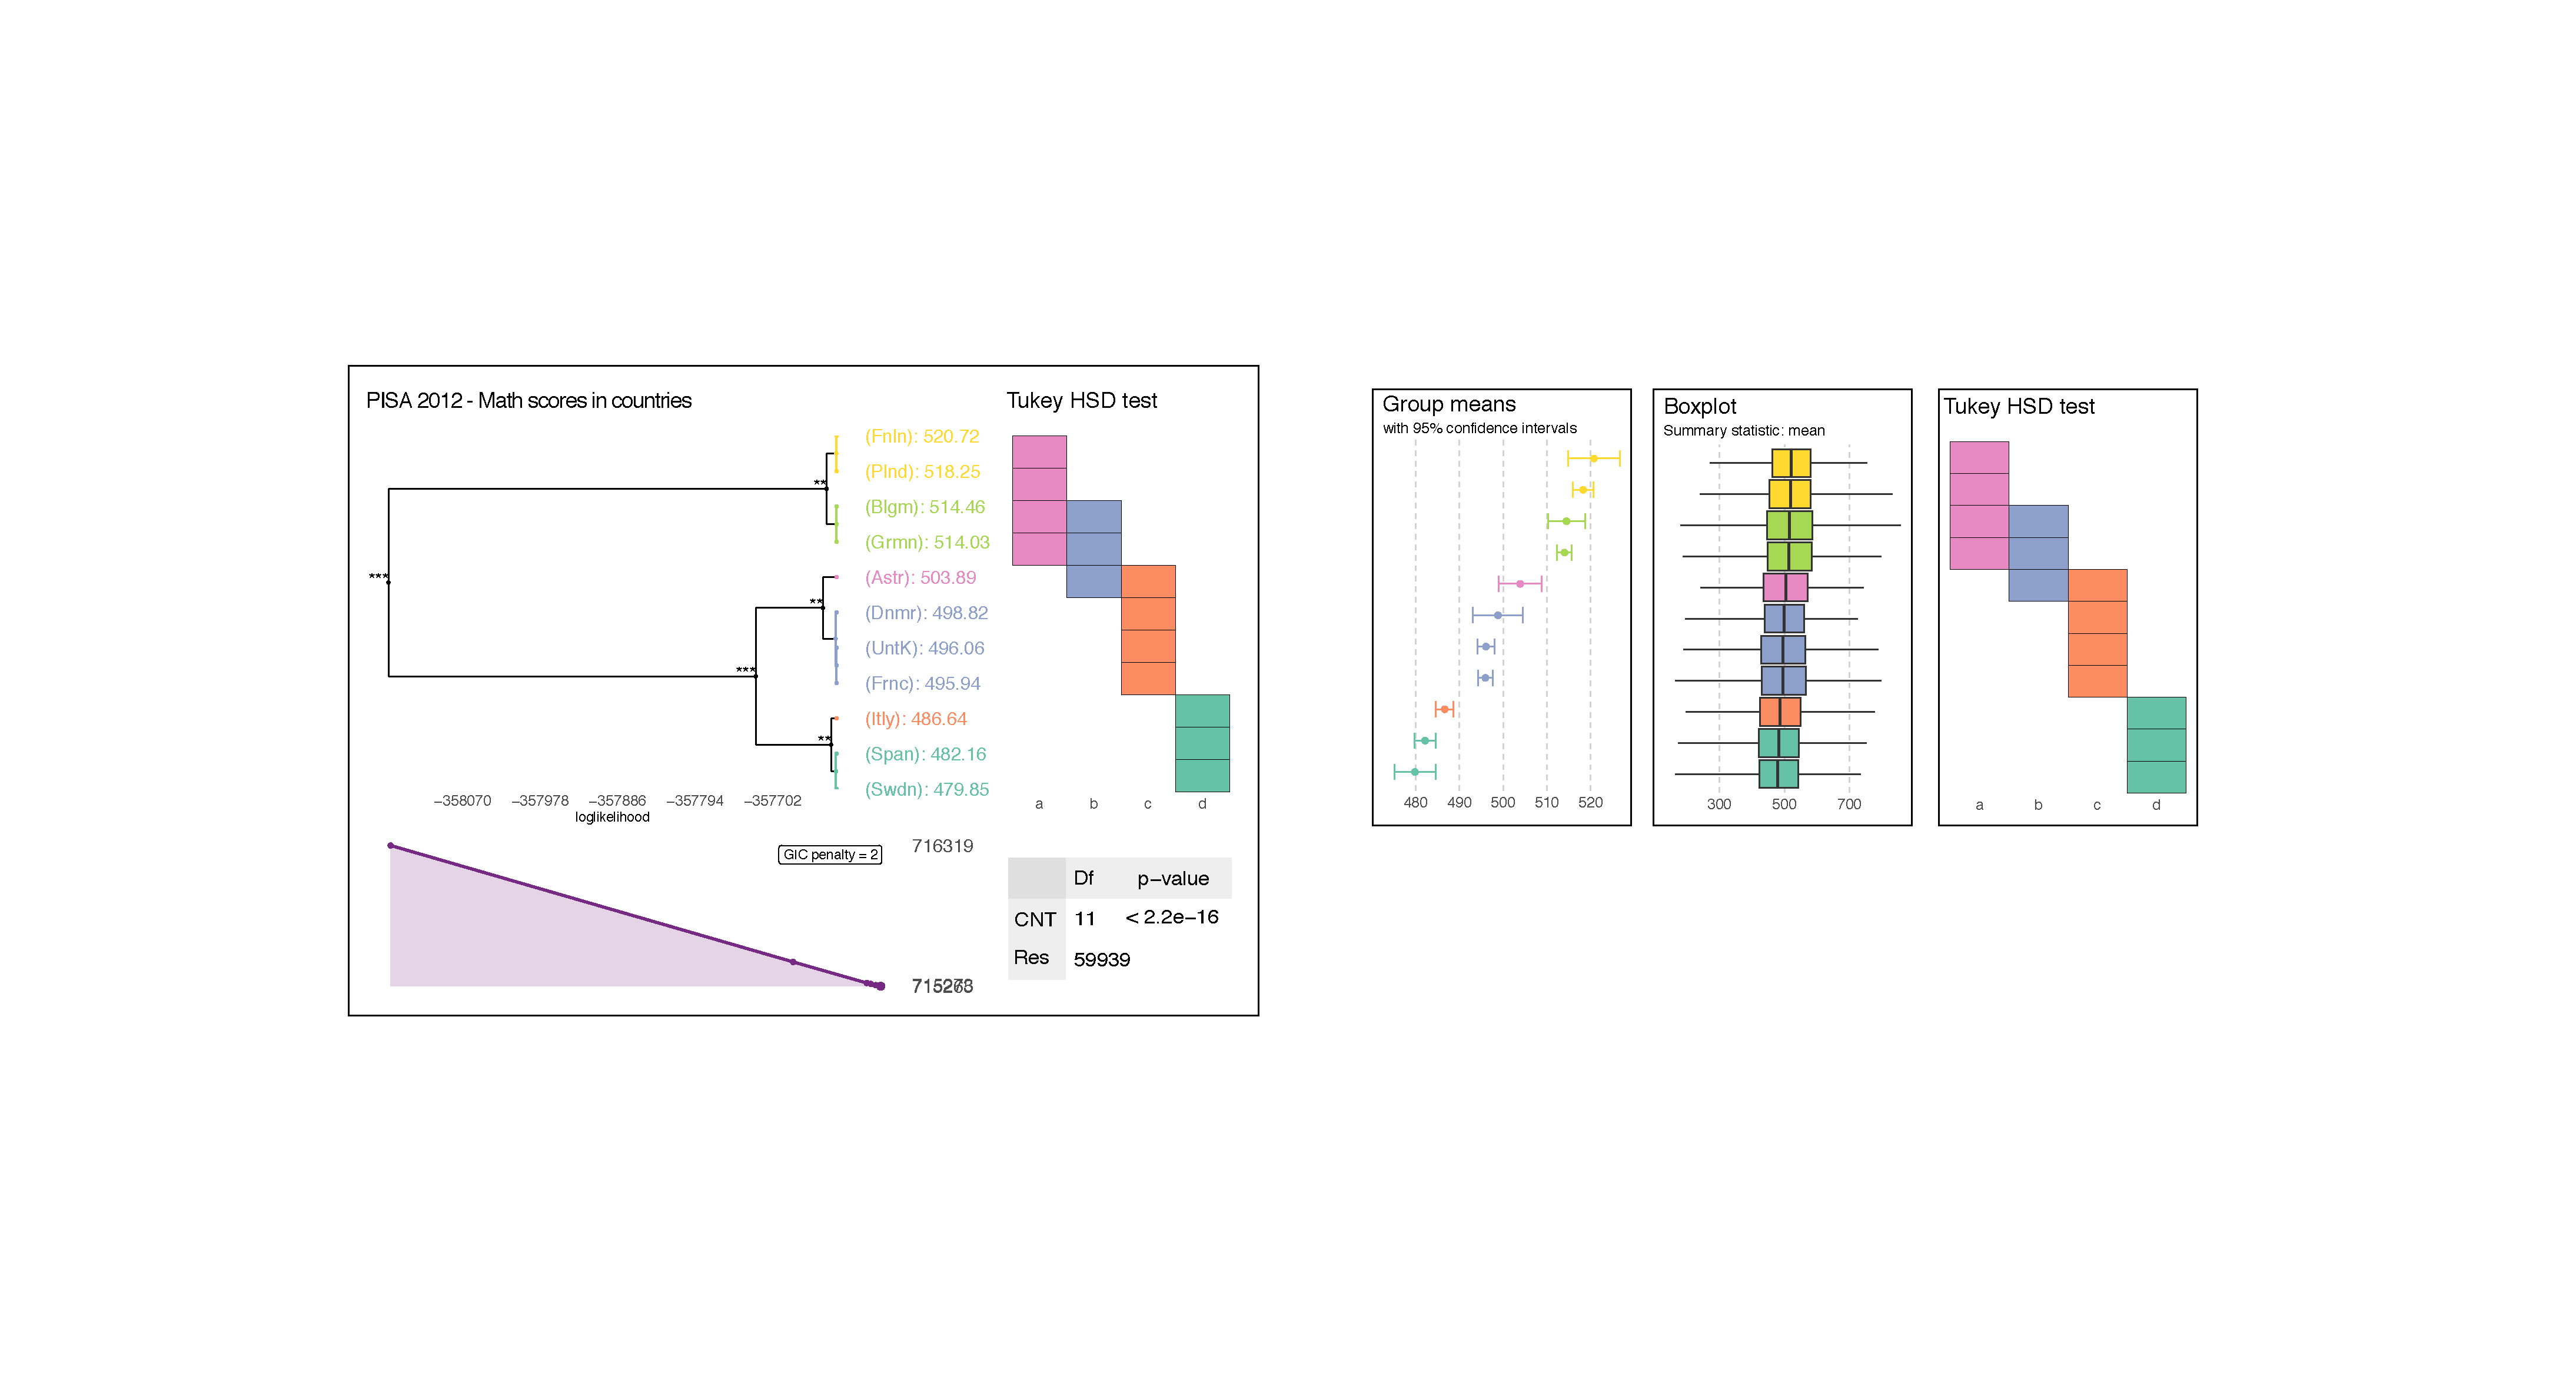
\includegraphics[width=\textwidth]{FM_tukey_done}
\caption{\label{fig:PISAtree}Four panels of \emph{Merging Paths Plot} for the PISA dataset for 11 countries. The panel A summaries the structure of group similarities. It shows the list of  models returned in the Algorithm 1. The OX axis presents values of log-likelihood function for each model from the list. Labels on the right margin presents averages of variable of interest for different groups. Stars in different joins of the tree summarizes pairwise tests for selected groups of variables. The panel B summaries the distribution of variable of interest in each group. The summary plotted in this panel may be changed depending of the model family. The panel C shows the Generalized Information Criteria for each model from the list. The Panel D presents results from the test for global null hypothesis. Colors in panels A and B are consistent and corresponds to optimal segmentation of groups based on GIC score.}
\end{figure}

\clearpage

The result of the algorithm 1 is the list of $k$ shrinking models $\mathcal{M}_i$, where $i \in \{1, ..., k\}$. These models are presented in a graphical way in a \emph{Merging Paths Plot} along with diagnostic criteria like Generalized Information Criteria  and graphical  summaries. 
The proposed plot contains four panels, that contain all important information in a compact form.
An example of these panels is presented in the Figure \ref{fig:PISAtree}.

The statistics presented in this plot are described in following subsections.

\subsection{Model families}

The Merging Paths Plots can be created for any likelihood based model.  Current version of the package supports following parametric models: 

\begin{itemize}
\item one-dimensional Gaussian (with the argument \code{family = "gaussian"}).  Here 
$$
y_{ij} \sim \mathcal{N}\left(\mu_{j}, \sigma^2\right)
$$
and corresponding logarithm of likelihood

$$
l\left(\mu, \sigma | y\right) = 
-\frac{n}{2} \log{\left(2\pi\right)} -\frac{n}{2} \log{\left(\sigma^2\right)} -\sum_{j=1}^k\sum_{i=1}^{n_j}\frac{1}{2}\left(y_{ij} - \mu_j\right)^2/ \sigma^2.
$$

Group summaries are averages -- maximum likelihood estimates for $\mu_j$.

\item n-dimensional Gaussian (with the argument \code{family = "gaussian"}). Here $Y_{ij}$ and $M_j$ are vectors and

$$Y_{ij} \sim \mathcal N \left(M_j, \Sigma\right).$$

The corresponding logarithm of likelihood function

$$
l\left(M, \Sigma | Y\right) = 
-\frac{n}{2} \log{\left(2\pi\right)} -\frac{n}{2} \log{\left(|\Sigma|\right)} -
\sum_{j=1}^k\sum_{i=1}^{n_j}\frac{1}{2}\left(Y_{ij} - M_j\right)^T\Sigma^{-1}\left(Y_{ij} - M_j\right).
$$

Note that, both one-dimensional and n-dimensional Gaussian models use \code{family = "gaussian"}. However, the visual summary of n-dimensional data requires additional preprocessing -- dimensionality reduction -- thus, it is considered as a~separate category.
Group summaries are averages.

\item binomial (with the argument \code{family = "binomial"}). Here
$$y_{ij} \sim \mathcal{B}\left(p_{j}, 1\right).$$
After adding the logit link function 
$$\ln\left(\frac{p_j}{1 - p_j}\right) = \beta_j$$
one may write the logarithm of likelihood

$$l\left(\beta|y\right) = \sum_{j=1}^k\sum_{i=1}^{n_j} y_{ij}\log\left(p_j\right) - (1 - y_{ij}) \log{\left(1 - p_j\right)}.$$

Group summaries are proportions of successes as estimates of $p$.

\item survival (with the argument \code{family = "survival"}). Here we consider the \emph{Cox proportional hazard model} \citep{coxph}.
Let $\lambda_0(t)$ be the baseline hazard function, where $t$ denotes time. Then the hazard function for group $j$ may be expressed as

$$
\lambda_j(t) = 
\lambda_0(t)\cdot \exp(\alpha_j).
$$

Corresponding logarithm of partial likelihood is

$$
l\left(\alpha\right|y) = 
	\sum_{i,j:C_{ij} = 1} 
		\left(
			\alpha_j -
			\log{
				\left(
				\sum_{kl:y_{kl}\geq y_{ij}} 
				\exp{\left(\alpha_k\right)}		
				\right)
			}
		\right).
$$
where $C_{ij}$ is the censoring status, $C_{ij} = 1$ means that the observation $i$ from group $j$ is not censored.
For this model hazard ratios are the group summaries.

\end{itemize}

The fusing algorithm that is used in \emph{Merging Paths Plots} is based on Likelihood Ratio Test statistic defined as

\begin{equation} \label{LRTstat}
LRT(\M_1;\M_2) = 2 \cdot l (\widehat{\beta_{\M_2}}|y) - 2 \cdot l (\widehat{\beta_{\M_1}}|y),
\end{equation}
where $\mathcal{M}_1$ and $\mathcal{M}_2$ are two nested models. Each model corresponds to a group of observations. Groups for both models are equal except that two groups in $\M_2$ are merged in a one group in $\M_1$.
The higher the $LRT(\M_1;\M_2)$, the more different were the merged groups. One may interpret the $LRT(\M_1;\M_2)$ as a distance between groups for model $\M_1$ and $\M_2$.

The advantage of \emph{LRT statistic} is the known asymptotic behavior \citep[see]{wilks1938large}. For models $\M_2$ a $\M_1$ that differs by one degree of freedom it holds
$$
LRT(\M_1;\M_2) \overset{n \rightarrow \infty}{\sim} \chi^2_1.
$$
This asymptotic distribution is used in \factorMerger to mark statistically significant group splits with the argument \code{panelGrid = TRUE} of the \code{plot.factorMerger} function. 

\subsection{Response panels}

The right panel of \emph{Merging Path Plots} shows graphical summaries of variable of interest in groups. Use the \texttt{responsePanel} argument to choose how groups shall be presented.

Available options are presented in the Figure \ref{fig:panele}. Depending on the family of the variable of interest different summaries are appropriate. Possible combinations are presented in 
the Table \ref{tab:responsePanelT}.

\begin{table}[H]
\centering 
\begin{tabular}[t]{c|c|c|c}
 \textbf{} & \textbf{} & \textbf{family} & \textbf{} \\
 \textbf{responsePanel} & \textbf{gaussian} & \textbf{binomial} & \textbf{survival} \\
\hline frequency & + & + & + \\
\hline means & + & &  \\
\hline boxplot & + & &  \\
\hline tukey & + & &  \\
\hline heatmap & + & &  \\
\hline profile & + & &  \\
\hline proportion & & + &  \\
\hline survival & & & + \\
\hline 
\end{tabular}
\caption{\label{tab:responsePanelT}Pluses denote which \texttt{responsePanel} may be used for which model family. Examples for each type of panel are presented in the Figure \ref{fig:panele}.}
\end{table}



\begin{figure}[h!tbp]
\centering
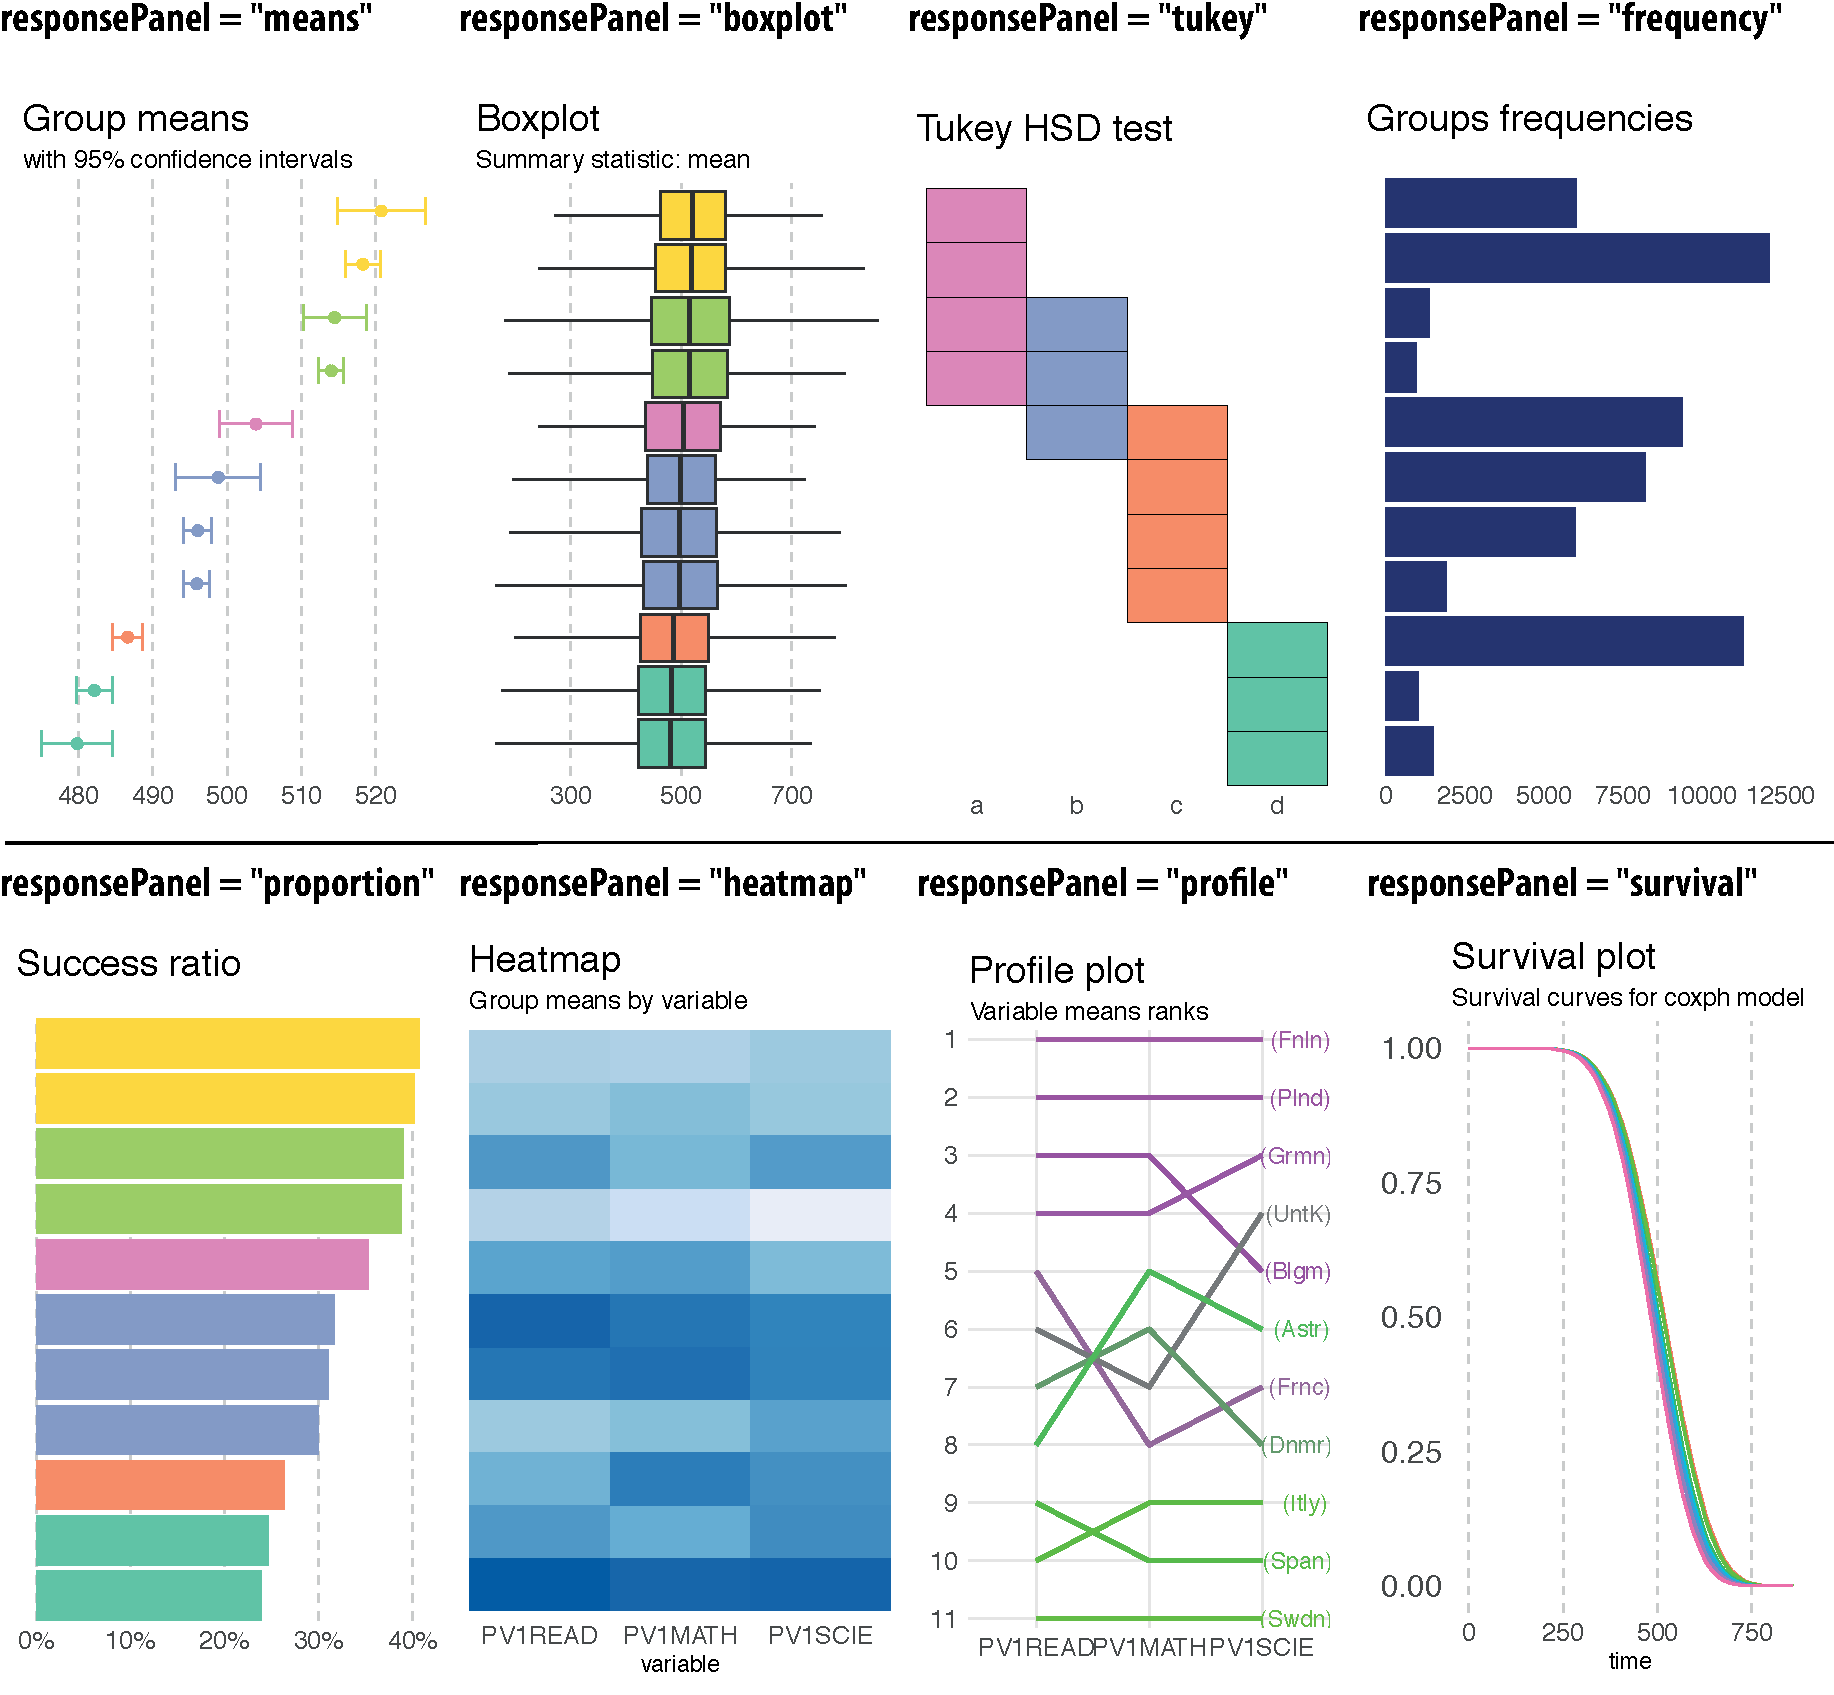
\includegraphics[width=\textwidth]{panelsWide}
\caption{\label{fig:panele}Avaliable options for the \texttt{responsePanel} argument. Different panels are designed to highlight different aspects of groups.}
\end{figure}


\clearpage

\subsection{General Information Criterion}

The fusing algorithm returns a collection of models of different size / different optimal number of groups. In order to select the best model the useful procedure is to select a model that minimize the Generalized Information Criteria
$$
GIC(\M) = -2 l(\M) + p |\M|
$$
where $|\M|$ denotes to number of groups in model $\M$ while $p$ is a penalty for model complexity. GIC corresponds to Akaike Information Criterion (AIC) for $p=2$ or Bayesian Information Criterion (BIC) for $p=\log(n)$.

To make it easier to select the best model the bottom-left panel presents the GIC plot. An example of such plot is presented in Figure \ref{fig:FM0}.

\begin{figure}[h!tbp]
\centering
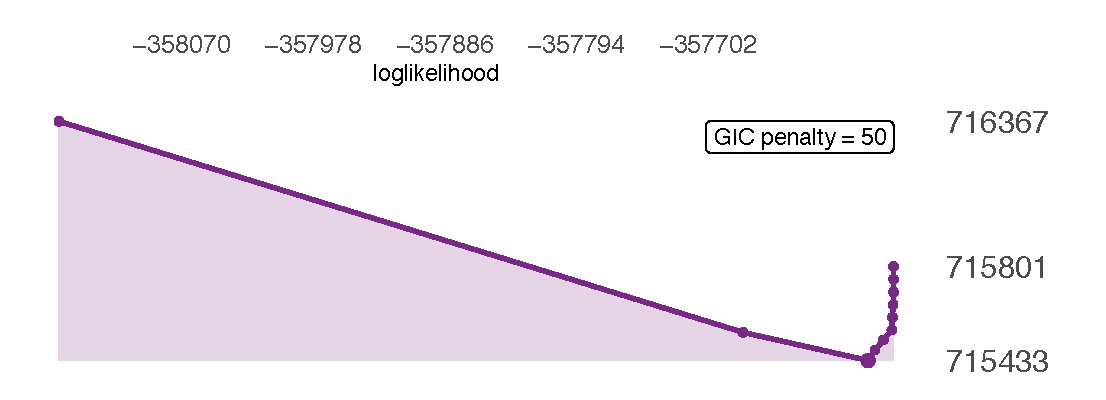
\includegraphics[width=0.75\textwidth]{FM_0}
\caption{\label{fig:FM0}
The GIC plot. OX axis corresponds to the log-likelihood for a model. OY axis corresponds to the GIC score for a model. GIC scores for the best, smallest and largest models are presented in the right axis.}
\end{figure}

\subsection{The Fusing Strategy}

The algorithm \ref{algorithm1} presents a general strategy for merging groups. The fully adaptive strategy is time consuming and may be slow for large number of groups. Thus in the \factorMerger package we have implemented four versions of the merging algorithm. These versions are summarized below.

Depending on the specific goal some steps of the Algorithm 1 may be performed differently. Possible options are:
\begin{itemize}
\item \texttt{fuse = {"}adaptive{"}}. The objective function is the logarithm of likelihood. The set $pairsSet$ contains all possible pairs of groups available in a given step. Pairwise LRT distances are recalculated every step. This option is the slowest one since it requires the largest number of comparisons. It requires $\text{O}(n^3)$ model evaluations.
\item \texttt{fuse = {"}fast-adaptive{"}}. 
Note that computing an objective function can be expensive and, especially for big datasets, it may be beneficial to limit the set of pairs that shall be compared. Also note that it is more likely that a~pair~of~levels $i$ and $j$ will be chosen to merge if~corresponding group averages are close. In this option, the objective function is the minimum logarithm of likelihood, but the $pairsSet$ is generated differently, in a following way. 
For Gaussian family of response, at the very beginning, the groups are ordered along of average values and then $pairsSet$ contains only pairs of closes groups. 
For other families the order corresponds to beta coefficients in a regression model. The detailed rules of ordering levels are given in the Table \ref{tab:ordering}.
This option is much faster than \texttt{fuse = {"}adaptive{"}} and requires $\text{O}(n^2)$ model evaluations.
\item \texttt{fuse = {"}fixed{"}}. This option is based on the DMR algorithm introduced in \cite{Proch}. It was extended to cover survival models. The largest difference between this option and the \texttt{fuse = {"}adaptive{"}} is, that in the first step a pairwise distances are calculated between each groups based on the $LRT$ statistic. Then the agglomerative clustering algorithm is used to merge consecutive pairs. It means that pairwise model differences are not recalculated as LRT statistics in every step but the \texttt{complete linkage} is used instead. 
This option is very fast and requires $\text{O}(n^2)$ comparisons.
\item \texttt{fuse = {"}fast-fixed{"}}. This option may be considered as a modification of \texttt{fuse = {"}fixed{"}}. The biggest difference is that in the first step we do not calculated whole matrix of pairwise differences, but instead only the differences between consecutive groups.
\end{itemize}

These options differ in two ways. First, they differ in terms of computational time. The fastest option is to calculated pairwise differences and then use complete-linkage hierarchical algorithm for fusions. The slowest option is to calculated pairwise differences between groups after each fusion. But also the slowest option is the best one, in terms that it gives groups with lowest log-likelihoods.

\begin{table}[H]
\centering \begin{tabular}[t]{c|p{9cm}}
\hline \textbf{family} & \textbf{ordering statistic for a given group} \\
\hline one-dimensional Gaussian & average in a group \\
\hline multi-dimensional Gaussian & average in a group after the Kruskal's non-metric multidimensional scaling \citep{MASS} to a one-dimensional space \\
\hline binomial & proportion of successes in a group\\
\hline survival & logarithm of a hazard ratio for a group\\
\hline 
\end{tabular}
\caption{\label{tab:ordering}Factor ordering by model family for \texttt{fuse = {"}fast-adaptive{"}}}
\end{table}

\todo{ASI: przenies opisy algorytmow do dokumentacji pakietu / funkcji mergeFactors}

\todo{ASI: umiesc informacje o czasach dzialania roznych algorytmow}

\todo{ASI: umiesc przyklad w korym fixed i adapive daja ine wyniki}


\clearpage










\section{Examples}
\label{sec:examples}

The \textbf{factorMerger} package is highly customizable through function arguments.
In this section we present four different case studies to illustrate the use of the \factorMerger in real examples. Each scenario is associated with a particular model family and also present additional graphical parameters in action. 

\subsection{Gaussian models}
\label{subsec:gauss}

\todo{Zacytowac PISA2012lite}

In the first two examples we use the \emph{PISA} (Program for International Student Assessment, 
\cite{pisa2012} \todo{zrodlo}) dataset which contains information on students' performance on various cognitive tests. Based on multiple survey results so-called \emph{plausible values} (\emph{zrodlo}) are modeled which resemble individual test scores. Those values are calculated in three different fields: mathematics,  normally distributed 

In this subsection we will continue with the PISA dataset described in \nameref{subsec:gauss}

\subsection{Binomial model}
\label{subsec:binom}

\begin{lstlisting}[language=R]
fib <- function(n) {
  if (n < 2)
    n
  else
    fib(n - 1) + fib(n - 2)
}
fib(10) # => 55
\end{lstlisting}

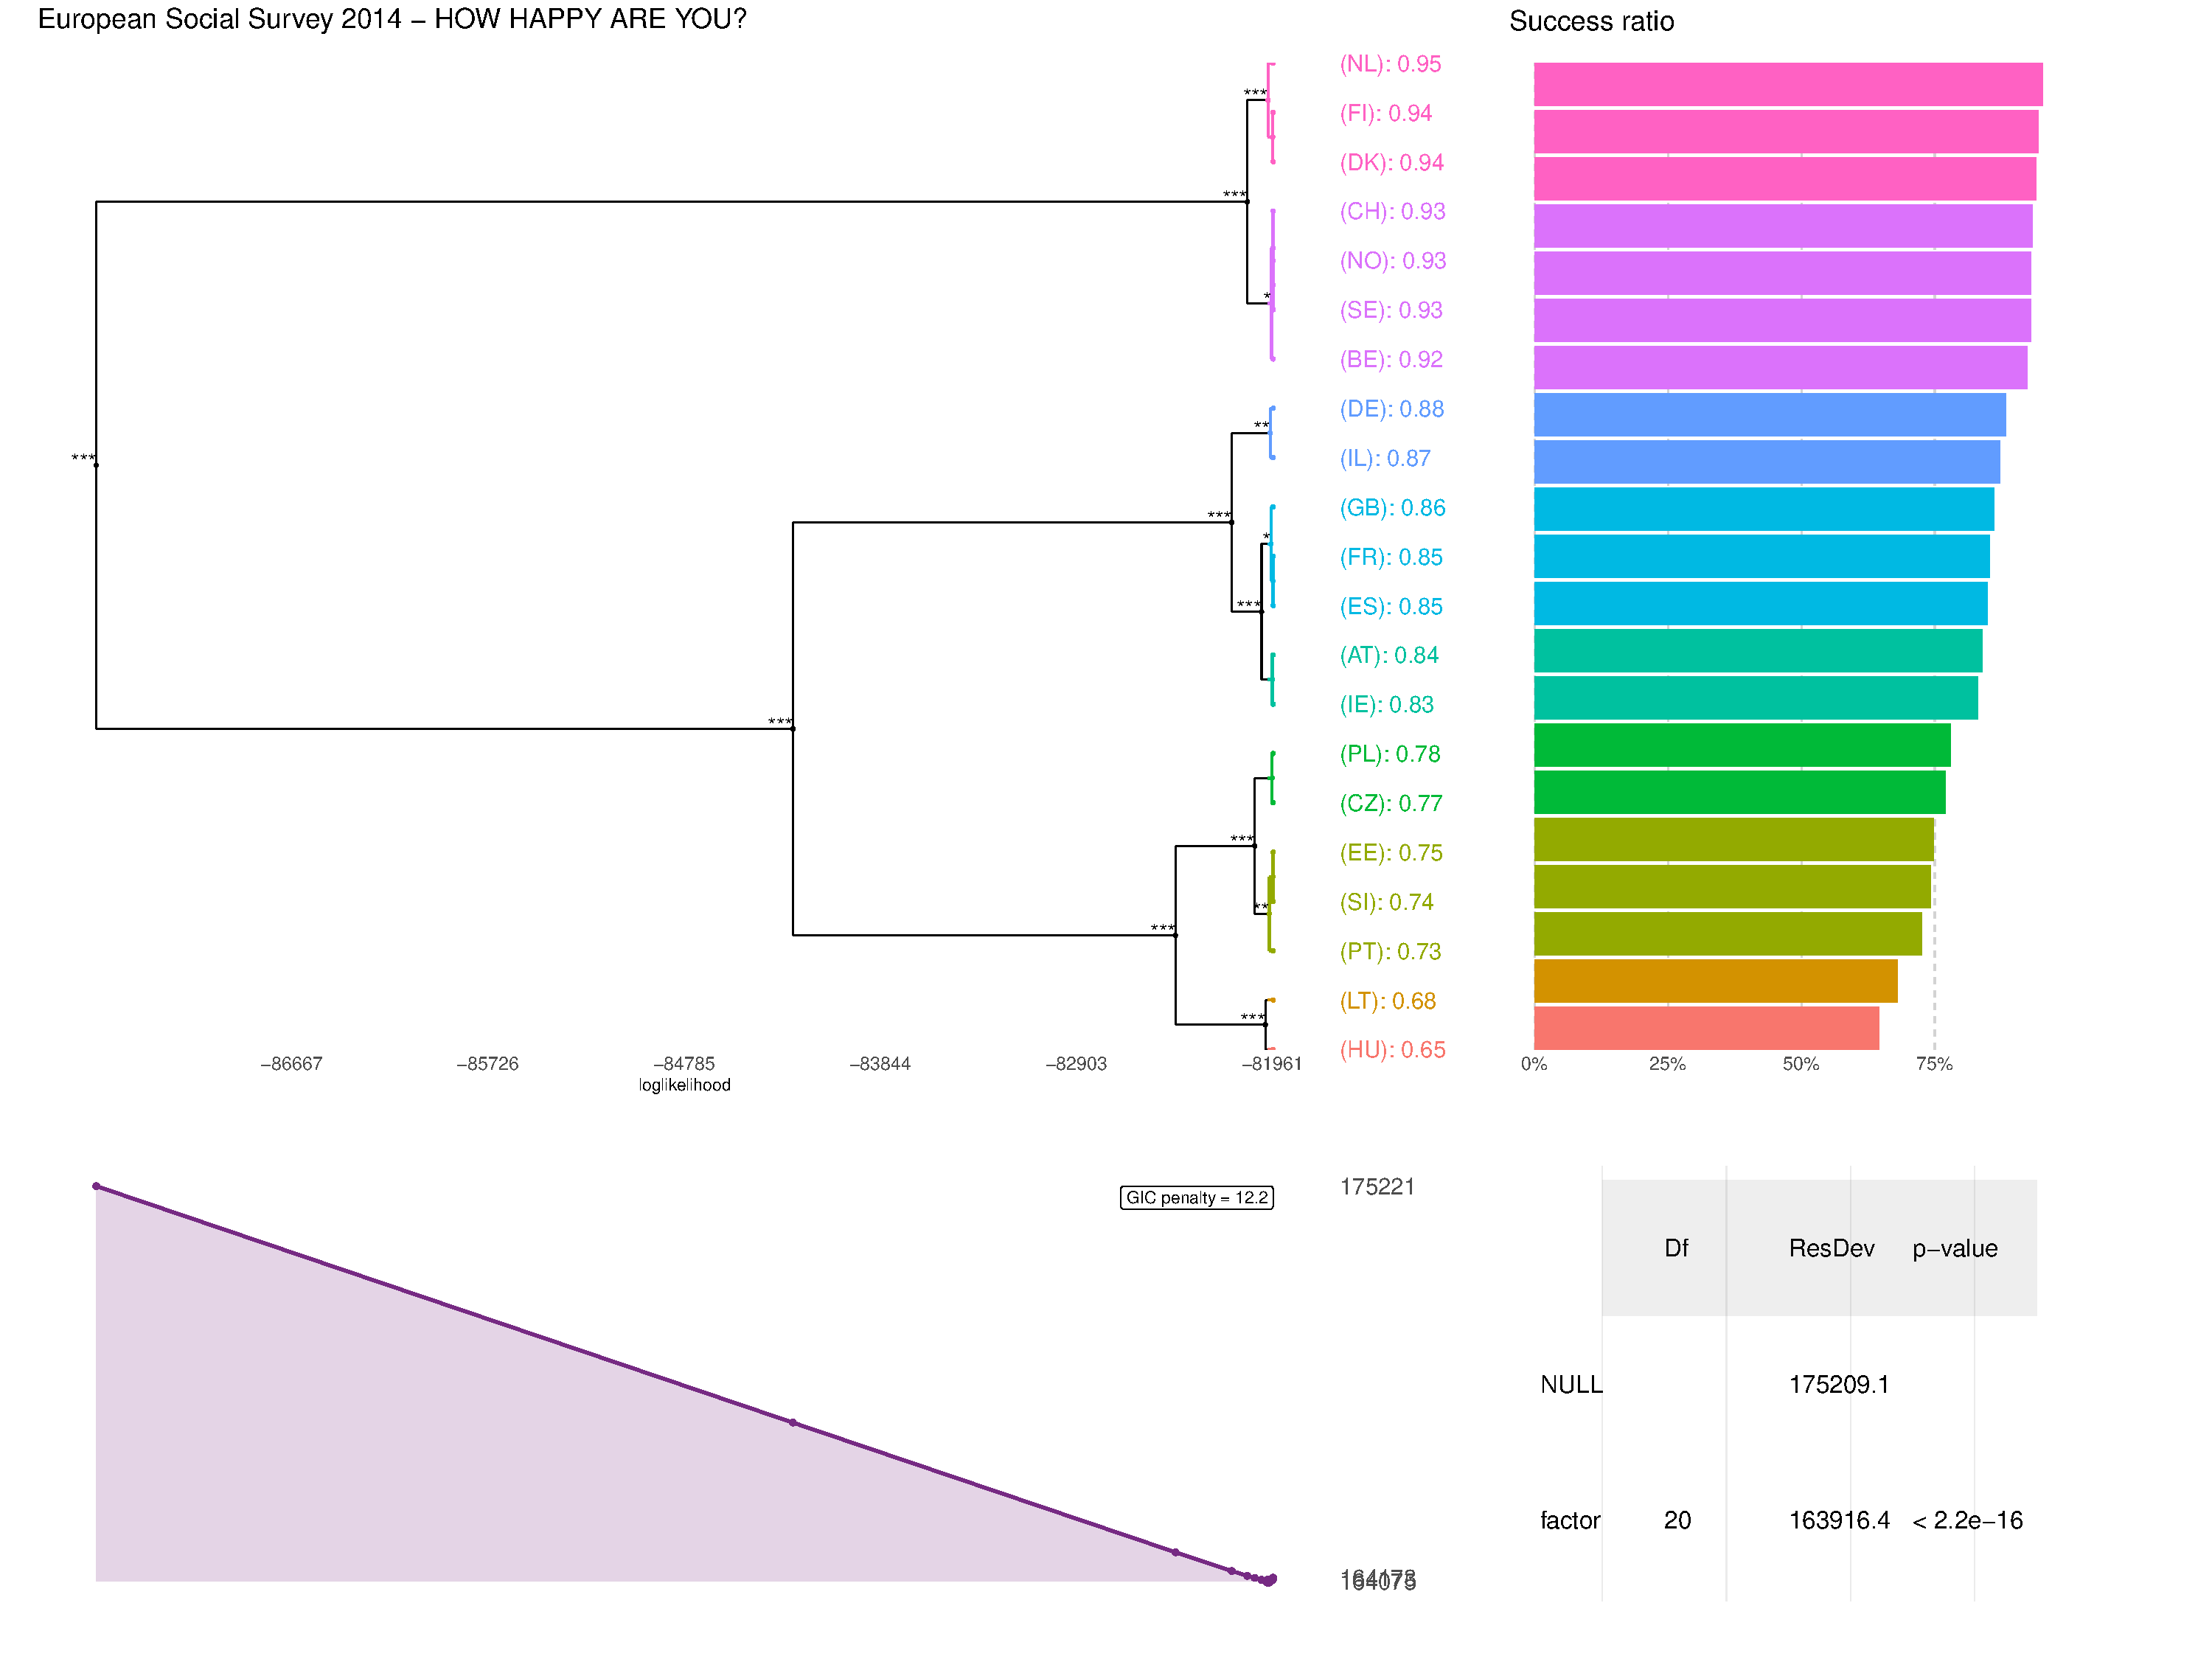
\includegraphics[scale=0.35]{ESS_FM2}

\subsection{Survival model}
\label{subsec:surv}


\section{Summary and Future Directions}
\label{sec:summ}

\emph{Merging Paths Plot} is a novel approach to summarize groups similarities based on LRT statistic. It is a useful tool to explore group similarities in k-sample problems.

In this article we have presented the methodology that is implemented in the \factorMerger R package.  Currently the implementation is limited to a single grouping variable, what correspond to a one-way ANOVA. The natural extension of this approach is related to more grouping variables possible with interactions. 

Other possible extensions are related to different classes of models. Instead of Likehood Ratio Test other tests for two - groups may be used. For example a Wilcoxon test may be used for semi-parametric modeling. 


\section{Acknowledgements}

We acknowledge the financial support from the \emph{NCN Opus grant 2016/21/B/ST6/02176}.

\todo{PBI: Wewnętrzne recenzje: BMIA? PTSE? APRO?}

\todo{PBI: Dodać uchwyty archivista}


\bibliographystyle{agsm}

\bibliography{sitko_biecek}
\end{document}
